\documentclass[a4paper,10pt]{report}
\usepackage[utf8]{inputenc}
\usepackage{graphicx}

% Title Page
\title{}
\author{}


\begin{document}

\section*{\textit{Layered Label Propagation Distribúido}(Esboço)}

Cada vértice terá:
\begin{itemize}
  \item A sua \textit{label}
  \item Pares \{$label_i$, $v_i$\} conhecidos até ao momento.
  \item Vértice adjacentes e \textit{labels} correspondentes.
\end{itemize}

\begin{figure}[h]
\center
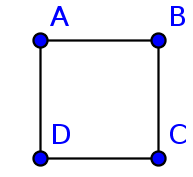
\includegraphics{graph_distributed_example1}
\caption{Primeiro grafo de exemplo.\label{fig:distributedexample1}}
\end{figure}

{\bf Exemplo para o grafo da figura \ref{fig:distributedexample1}}
\\[0.25cm]
{\bf Fase de preparação:}\\
Todos os vértices mandam para os seus adjacentes informação sobre a sua \textit{label} e com $v_i=1$. 
\\[0.25cm]
{\bf 1ª iteração (com $\gamma=1$):}
\\[0.25cm]
Vértice A:
  \begin{tabular}{| l | l | l | l |}
  \hline
  $label_i$ & $k_i$ & $v_i$ conhecido & $k_i - \gamma(v_i - k_i)$\\ \hline
  A & 0 & 1 & -1 \\ \hline
  B & 1 & 1 & 1 \\ \hline
  D & 1 & 1 & 1 \\ \hline
  \end{tabular}
  A fica com a \textit{label} B.
\\[0.25cm]
Vértice B:
  \begin{tabular}{| l | l | l | l | l |}
  \hline
  $label_i$ & $k_i$ & $v_i$ conhecido & $k_i - \gamma(v_i - k_i)$\\ \hline
  A & 1 & 1 & 1 \\ \hline
  B & 0 & 1 & -1 \\ \hline
  C & 1 & 1 & 1 \\ \hline
  \end{tabular}
  B fica com a \textit{label} A.
\\[0.25cm]
Vértice C:
  \begin{tabular}{| l | l | l | l |}
  \hline
  $label_i$ & $k_i$ & $v_i$ conhecido & $k_i - \gamma(v_i - k_i)$\\ \hline
  B & 1 & 1 & 1 \\ \hline
  C & 0 & 1 & -1 \\ \hline
  D & 1 & 1 & 1 \\ \hline
  \end{tabular}
  C fica com a \textit{label} B.
\\[0.25cm]
Vértice D:
  \begin{tabular}{| l | l | l | l |}
  \hline
  $label_i$ & $k_i$ & $v_i$ conhecido & $k_i - \gamma(v_i - k_i)$\\ \hline
  A & 1 & 1 & 1 \\ \hline
  C & 1 & 1 & 1 \\ \hline
  D & 0 & 1 & -1 \\ \hline
  \end{tabular}  
  D fica com a \textit{label} A.
  
  \newpage
  
  {\bf 2ª iteração (com $\gamma=1$):}
\\[0.25cm]
Vértice A:
  \begin{tabular}{| l | l | l | l |}
  \hline
  $label_i$ & $k_i$ & $v_i$ conhecido & $k_i - \gamma(v_i - k_i)$\\ \hline
  A & 2 & 2 & 2 \\ \hline
  B & 0 & 1 & -1 \\ \hline
  D & 0 & 0 & 0 \\ \hline
  \end{tabular}
  A fica com a \textit{label} A.
\\[0.25cm]
Vértice B:
  \begin{tabular}{| l | l | l | l |}
  \hline
  $label_i$ & $k_i$ & $v_i$ conhecido & $k_i - \gamma(v_i - k_i)$\\ \hline
  A & 0 & 1 & -1 \\ \hline
  B & 2 & 2 & 2 \\ \hline
  C & 0 & 0 & 0 \\ \hline
  \end{tabular}
  B fica com a \textit{label} B.
\\[0.25cm]
Vértice C:
  \begin{tabular}{| l | l | l | l |}
  \hline
  $label_i$ & $k_i$ & $v_i$ conhecido & $k_i - \gamma(v_i - k_i)$\\ \hline
  A & 2 & 2 & 2 \\ \hline
  B & 0 & 1 & -1 \\ \hline
  C & 0 & 0 & 0 \\ \hline
  D & 0 & 0 & 0 \\ \hline
  \end{tabular}
  C fica com a \textit{label} A.
\\[0.25cm]
Vértice D:
  \begin{tabular}{| l | l | l | l |}
  \hline
  $label_i$ & $k_i$ & $v_i$ conhecido & $k_i - \gamma(v_i - k_i)$\\ \hline
  A & 1 & 1 & 1 \\ \hline
  C & 1 & 1 & 1 \\ \hline
  D & 0 & 1 & -1 \\ \hline
  \end{tabular}
  C fica com a \textit{label} B.
  
  
  
\end{document}          
